% !TEX program = xelatex
\documentclass[11pt,a4paper]{amsart}
\usepackage[margin=30mm]{geometry}
\usepackage{amsmath,amssymb,mathtools}
\usepackage[no-math]{fontspec}
\setmainfont{Latin Modern Roman}[SmallCapsFont={Latin Modern Roman Caps}]
\IfFontExistsTF{Noto Serif CJK JP}
  {\newfontfamily\japanesefont{Noto Serif CJK JP}[Scale=.9]}
  {\IfFontExistsTF{Yu Gothic}
    {\newfontfamily\japanesefont{Yu Gothic}[Scale=.9]}
    {\newfontfamily\japanesefont{MS Gothic}[Scale=.9]}}
\newcommand{\jp}[1]{{\japanesefont #1}}
\usepackage{booktabs,tikz,needspace}
\usetikzlibrary{arrows.meta,decorations.pathreplacing}
\usepackage[hidelinks,unicode]{hyperref}
\hypersetup{pdftitle={Interruption Timing under Hidden Information: Sharp Bounds on Conflicting States},pdfsubject={Finite resource allocation and Helly-type theorems}}
\newtheorem{theorem}{Theorem}[section]
\newtheorem{lemma}[theorem]{Lemma}
\newtheorem{proposition}[theorem]{Proposition}
\newtheorem{corollary}[theorem]{Corollary}
\theoremstyle{definition}
\newtheorem{definition}[theorem]{Definition}
\theoremstyle{remark}
\newtheorem{remark}[theorem]{Remark}
\newcommand{\N}{\mathbb N}
\newcommand{\Safe}{\operatorname{Safe}}
\newcommand{\Feas}{\operatorname{Feas}}
\newcommand{\card}[1]{\lvert #1\rvert}
\newcommand{\cardnote}[2]{\footnote{Japanese card name: \href{https://www.db.yugioh-card.com/yugiohdb/card_search.action?ope=2\&cid=#1\&request_locale=ja}{\jp{#2}}.}}
\date{}
\keywords{Hidden information, interruption timing, finite resources, Helly-type theorem, minimal obstruction, hypergraph}
\title[Resource bounds for hidden-state conflicts]{Interruption Timing under Hidden Information:\ Sharp Bounds on Conflicting States}

\begin{document}
\begin{abstract}
A defender can spend a resource before an irreversible deadline or retain it
for a later threat whose target becomes observable. We study this trade-off
in a finite model motivated by a graveyard-removal decision in Yu-Gi-Oh!
Each hidden state specifies urgent targets, a pool of later targets, and a
bound on the number of distinct late requests. Every removal consumes one unit
from a shared budget. We derive the exact minimum budget and prove that every
family infeasible at budget $k$ contains an infeasible subfamily of at most
$k+1$ states. If every state has late demand at least $d$ after the canonical
early action, the bound improves to $1+\max\{k-d,0\}$. Both bounds are sharp.
A three-state example is pairwise feasible but jointly infeasible and shows
that the budget function can violate submodularity and LP-type locality.
When one action can remove several targets, minimal obstructions can be
arbitrarily large even at budget one. These results show how the granularity
of a resource controls the order of conflicts under hidden information.
\end{abstract}
\maketitle

\section{Introduction}

An interruption has value both for the threat it can stop immediately and
for the threat it may stop after an opponent reveals a continuation. Under
hidden information, the same public position can support continuations that
favor different timings. The defender must allocate a shared stock of resources
across requirements that are individually manageable but jointly incompatible.

Yu-Gi-Oh! supplies a concrete example. D.D. Crow\cardnote{6980}{D.D.クロウ}
can remove a card from the opponent's graveyard in response to an effect.
Using it before a revival resolves can stop an immediate attack; keeping it
can stop a later revival once its target is announced. Acting early consumes
the resource, whereas waiting can let the original target leave the zone
where Crow is effective. Section~\ref{sec:cards} gives a position in which an
unknown hand card determines which timing wins.

This position leads to a question about the size of a conflict:
if a family of hidden states cannot be defended with $k$ interruptions, how
many states are needed to witness that failure? We address this question
for a two-stage removal model. A hidden state $\theta$ specifies an urgent
set $U_\theta$, a late target pool $L_\theta$, and a late-request quota
$r_\theta$. The defender chooses one early removal set for all possible
states and subsequently responds to observed targets. Every target costs
one unit to remove.

For a finite information class $B$, write
$U_B=\bigcup_{\theta\in B}U_\theta$. We show that its minimum required budget is
\begin{equation}\label{eq:introthreshold}
 \kappa(B)=\card{U_B}+
 \max_{\theta\in B}\min\{r_\theta,\card{L_\theta\setminus U_B}\},
\end{equation}
where the maximum over the empty set is zero. The principal result is the
sharp implication
\[
 \kappa(B)>k\quad\Longrightarrow\quad
 \exists C\subseteq B:\ \card C\le k+1\ \text{and}\ \kappa(C)>k.
\]
The proof associates urgent targets with the states that require them and,
when necessary, adds one state witnessing excessive late demand. A uniform
lower bound on late demand after the canonical early action sharpens the bound.

The model is a two-stage robust decision problem: an initial commitment
is followed by an adaptive response to uncertainty~\cite{goerigk,kasperski}.
Equal single-target costs yield a canonical early action and a sharp bound on
conflicting states. This Helly-type bound relates global infeasibility to small
infeasible subfamilies~\cite{amenta,amentathesis,cardinal}. Minimal obstructions
also describe which states can share a successful signal, as in hypergraph
formulations of information compatibility~\cite{yuan}. The main contribution
is the sharp bound on obstruction size in terms of the removal budget and
the residual demand after the canonical early action. The higher-order
examples further describe the structure of this feasibility system.

\section{A graveyard-removal decision}\label{sec:cards}

Consider the following response window in Main Phase~1 of the attacker's turn.
The defender has $4000$ Life Points, an empty field, and a hand consisting of
D.D. Crow and Ookazi.\cardnote{4352}{昼夜の大火事}
The attacker has $800$ Life Points and has activated a previously set
Call of the Haunted,\cardnote{4989}{リビングデッドの呼び声}
targeting a particular copy $b_1$ of
Blue-Eyes White Dragon\cardnote{4007}{青眼の白龍}
in the attacker's graveyard. That graveyard contains all three copies
$b_1,b_2,b_3$ and a Blue-Eyes Ultimate Dragon\cardnote{4386}{青眼の究極竜}
that was properly Fusion Summoned before being sent there. The attacker
controls no monsters, and Call is the only card on either field. It is
Chain Link~1, with the defender next to respond. The defender's graveyard
contains no monsters. Both decks are nonempty and both Extra Decks are
empty. All other cards and effects are inactive throughout the continuation.

The attacker's only hand card is either
Axe of Despair\cardnote{4310}{デーモンの斧}
or Monster Reborn.\cardnote{4842}{死者蘇生}
These two hands define the information class for the decision.
The two states share a public history: exchanging the unrevealed card with
its alternative in the remaining deck leaves all earlier revealed actions
unchanged. The defender drew Ookazi during the current Standby Phase
through a previously set Jar of Greed,\cardnote{5210}{強欲な瓶}
so it first became available during the attacker's turn.
The card effects and response windows are specified in the official card
database and timing guide~\cite{konami,timing}.

Two defensive policies illustrate the timing conflict. The \emph{early} policy
chains Crow to Call and removes $b_1$. The \emph{reserved} policy lets Call
resolve and retains Crow to remove the target of a subsequent Monster
Reborn. In either policy, the defender activates Ookazi on the next turn
if that turn is reached.

\begin{center}
\begin{tabular}{lcc}
\toprule
Defensive policy & Hidden Axe & Hidden Reborn\\
\midrule
Remove $b_1$ immediately & Defender wins & Attacker can win\\
Reserve Crow for Reborn & Attacker can win & Defender wins\\
\bottomrule
\end{tabular}
\end{center}

Against Axe, early removal leaves the attacker without a monster. If Call
resolves instead, the revived White Dragon gains $1000$ ATK and deals
$4000$ damage. Against Reborn, early removal permits the later revival of
Ultimate Dragon, whose $4500$ ATK is lethal. Reserving Crow removes Reborn's
announced target before resolution and leaves at most the original
$3000$-ATK attacker. The defender then survives and wins with Ookazi's
$800$ damage. Reborn chooses its target before Crow is discarded, and the
defender's graveyard initially contains no monster that could serve as an
alternative target.

Other early targets do not resolve the conflict. Removing any card other
than $b_1$ leaves the Axe line intact. Against Reborn, removing Ultimate
Dragon still permits a second White Dragon to join $b_1$, for $6000$ total
attack damage; removing another card leaves Ultimate Dragon available.
Consequently, with one Crow the defender has a winning policy in each fully
specified state, but no single policy guarantees victory in both. Two Crows suffice:
remove $b_1$ first and reserve the second for a later revival from the
attacker's graveyard. Reborn can alternatively summon the defender's
discarded Crow, whose $100$ ATK is nonlethal.

The position illustrates competition between urgent and deferred uses of the
same resource. In the model below, each unanswered target causes failure and
each removal costs one unit. This formulation isolates the resource interaction
from the attack-damage calculation in the card position.

\section{The removal model and its exact threshold}\label{sec:model}

Let $X$ be a set of targets and $\Theta$ a set of hidden states. For each
$\theta\in\Theta$, let $U_\theta,L_\theta\subseteq X$ be finite sets and
let $r_\theta\in\N$, where $0\in\N$. The defender knows a finite information
class $B\subseteq\Theta$ and has $k\in\N$ identical removal units.
For nonempty $B$, a state $\theta\in B$ is fixed throughout play and hidden
from the defender. Every target in the specified sets is available for early
removal; the uncertainty concerns which requirements will apply.

Before an urgent deadline, the defender chooses a finite set $E\subseteq X$
and spends $\card E$ units. The same $E$ is used in every state in $B$.
In the actual state $\theta$, every urgent target must belong to $E$.
After the deadline, the adversary may request up to $r_\theta$ distinct
targets from $L_\theta\setminus E$, one at a time. The defender observes
each requested target and spends one unit to remove it. An unanswered
urgent or late target causes failure. Removed targets remain removed,
and spent units are not replenished. Figure~\ref{fig:timing} shows the timing.

\begin{figure}[htbp]
\centering
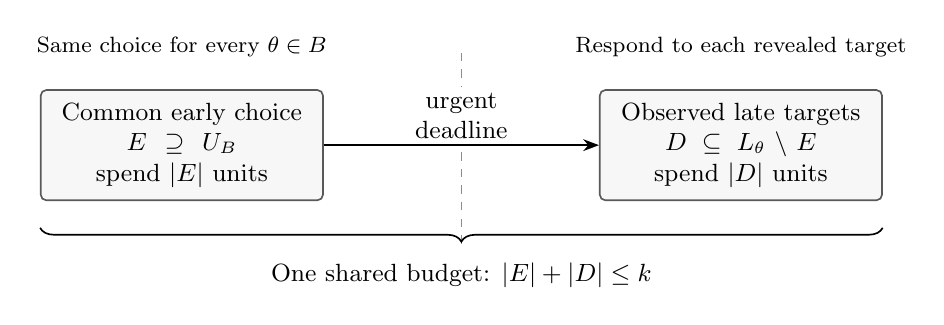
\begin{tikzpicture}[font=\small,>=Stealth,
  stage/.style={draw=black!65,rounded corners=2pt,align=center,minimum height=1.4cm,text width=3.35cm,fill=black!3},
  every path/.style={line width=.6pt}]
\node[stage] (early) at (0,0) {Common early choice\\$E\supseteq U_B$\\spend $|E|$ units};
\node[stage] (late) at (7.1,0) {Observed late targets\\$D\subseteq L_\theta\setminus E$\\spend $|D|$ units};
\draw[dashed,black!45] (3.55,-1.25) -- (3.55,1.25);
\draw[->] (early.east) -- node[above,align=center,fill=white,inner sep=2pt] {urgent\\deadline} (late.west);
\node[font=\footnotesize,align=center] at (0,1.25) {Same choice for every $\theta\in B$};
\node[font=\footnotesize,align=center] at (7.1,1.25) {Respond to each revealed target};
\draw[decorate,decoration={brace,mirror,amplitude=5pt}] (-1.8,-1.05) -- (8.9,-1.05);
\node at (3.55,-1.65) {One shared budget: $|E|+|D|\le k$};
\end{tikzpicture}


\caption{The early choice is common to the information class. Later
responses use the identities of the requested targets. Both stages draw
on the same budget.}
\label{fig:timing}
\end{figure}

\begin{definition}
An early set $E$ is \emph{safe for $B$ at budget $k$} if $\card E\le k$ and,
for every $\theta\in B$,
\begin{equation}\label{eq:safe}
 U_\theta\subseteq E,
 \qquad
 \card E+\card D\le k
 \quad\text{for every }D\subseteq L_\theta\setminus E
 \text{ with }\card D\le r_\theta.
\end{equation}
The family $B$ is \emph{feasible at budget $k$} if it has a safe early set.
Its minimum feasible budget is denoted by $\kappa(B)$.
\end{definition}

A finite feasible budget always exists: remove $U_B$ early and retain
enough units for the largest remaining late pool. In particular,
$\kappa(\varnothing)=0$.

The safety definition characterizes successful sequential defense.
If it holds, spending one unit on each observed request succeeds against
every sequence, including adaptively chosen sequences. Conversely, early
expenditure exceeding $k$ is inadmissible, and a missed urgent target
causes failure at the deadline. In the remaining case, failure of safety
provides a state and a legal set $D$ with $\card E+\card D>k$. Requesting
its elements in any order forces an unanswered request. Observing the
requested targets therefore suffices for a successful response policy.

\begin{lemma}\label{lem:cost}
For fixed $\theta$ and $E$, the early expenditure plus the largest
admissible late demand is
\begin{equation}\label{eq:cost}
 c_\theta(E)=\card E+\min\{r_\theta,\card{L_\theta\setminus E}\}
 =\min\{\card E+r_\theta,\card{E\cup L_\theta}\}.
\end{equation}
If $E\subseteq F$, then $c_\theta(E)\le c_\theta(F)$.
\end{lemma}
\begin{proof}
The adversary can request exactly
$\min\{r_\theta,\card{L_\theta\setminus E}\}$ remaining targets and cannot
request more. The second equality follows from
$\card{E\cup L_\theta}=\card E+\card{L_\theta\setminus E}$.
Both arguments of the final minimum are nondecreasing as $E$ grows,
which proves monotonicity.
\end{proof}

\begin{theorem}[Exact threshold]\label{thm:threshold}
For every finite $B\subseteq\Theta$, formula~\eqref{eq:introthreshold} holds.
In particular, $B$ is feasible at budget $k$ if and only if
$\kappa(B)\le k$.
Whenever $B$ is feasible at budget $k$, the early set $E=U_B$ is safe at
that budget.
\end{theorem}
\begin{proof}
Every safe early set contains $U_B$. By Lemma~\ref{lem:cost}, replacing
such a set by $U_B$ weakly decreases the total cost in every state and
also weakly decreases early expenditure. Thus $U_B$ is an optimal early
set. Taking the maximum late demand over $B$ gives the formula. For the
empty family, both terms are zero.
\end{proof}

\begin{corollary}\label{cor:mono}
If $C\subseteq B$, then $\kappa(C)\le\kappa(B)$.
\end{corollary}
\begin{proof}
Every early set safe for $B$ is safe for $C$ at the same budget.
\end{proof}

The canonical action has a simple interpretation: an extra early removal
can save at most the one unit it costs later. Removing every possible urgent
target and deferring all other removals therefore attains the minimum
worst-case budget.

\section{Sharp bounds on infeasible subfamilies}\label{sec:bounds}

\begin{lemma}[Selecting witnesses]\label{lem:witness}
If $S\subseteq U_B$, then there is a subfamily $C\subseteq B$ such that
$S\subseteq U_C$ and $\card C\le\card S$.
\end{lemma}
\begin{proof}
For each $x\in S$, choose a state $\theta_x\in B$ with $x\in U_{\theta_x}$,
and take $C=\{\theta_x:x\in S\}$.
\end{proof}

\begin{theorem}[Sharp obstruction bound]\label{thm:helly}
For every finite $B\subseteq\Theta$ and every $k\in\N$,
\begin{equation}\label{eq:helly}
 \kappa(B)>k
 \quad\Longleftrightarrow\quad
 \exists C\subseteq B:\ \card C\le k+1\ \text{and}\ \kappa(C)>k.
\end{equation}
For every $k$, the bound $k+1$ is attained by an inclusion-minimal
infeasible family.
\end{theorem}
\begin{proof}
The reverse implication follows from Corollary~\ref{cor:mono}. For the
forward implication, first suppose $\card{U_B}>k$. Choose
$S\subseteq U_B$ of size $k+1$ and apply Lemma~\ref{lem:witness}.
The resulting $C$ has at most $k+1$ states and requires at least $k+1$
early removals, so $\kappa(C)>k$.

Now suppose $\card{U_B}\le k$. By Theorem~\ref{thm:threshold}, some
$\theta_*\in B$ satisfies $c_{\theta_*}(U_B)>k$. Apply
Lemma~\ref{lem:witness} to $S=U_B$, obtaining a family $C_0$ of at most
$\card{U_B}$ states whose urgent union is $U_B$. Set
$C=C_0\cup\{\theta_*\}$. Then $U_C=U_B$ and $\theta_*\in C$,
so the same excessive late cost persists in $C$. Moreover,
$\card C\le\card{U_B}+1\le k+1$.

For sharpness, take $k+1$ states indexed by $i$, with $U_i=\{i\}$,
$L_i=\varnothing$, and $r_i=0$. Every subfamily $C$ has
$\kappa(C)=\card C$. Thus the full family is infeasible and every
proper subfamily is feasible at budget $k$.
\end{proof}

Equivalently, feasibility of all subfamilies of size at most $k+1$
implies feasibility of the whole family. The bound is independent of
the number of available states and target labels.

\begin{definition}
A number $d\in\N$ is a \emph{uniform late reserve for $B$} if
\begin{equation}\label{eq:reserve}
 d\le\min\{r_\theta,\card{L_\theta\setminus U_B}\}
 \qquad\text{for every }\theta\in B.
\end{equation}
\end{definition}

The reserve is measured at the canonical early set $E=U_B$. Removing
additional late targets early can reduce later demand, but
Lemma~\ref{lem:cost} shows that it cannot reduce the combined expenditure.
If $C\subseteq B$, then
$U_C\subseteq U_B$, so~\eqref{eq:reserve} also holds for each
$\theta\in C$ with $U_C$ in place of $U_B$.

\begin{theorem}[Reserve refinement]\label{thm:reserve}
Suppose $d$ is a uniform late reserve for $B$. If $\kappa(B)>k$, then
there is a subfamily $C\subseteq B$ such that
\[
 \kappa(C)>k,
 \qquad \card C\le 1+\max\{k-d,0\}.
\]
The bound is sharp for every pair $k,d\in\N$.
\end{theorem}
\begin{proof}
An infeasible family is nonempty. If $d>k$, any singleton from $B$
already has late demand exceeding $k$ and supplies the required witness.
Suppose henceforth that $d\le k$.

If $\card{U_B}+d>k$, choose $k-d+1$ urgent targets and select their
witness states by Lemma~\ref{lem:witness}. The resulting nonempty family
$C$ satisfies $\card C\le k-d+1$ and $\card{U_C}\ge k-d+1$.
The inherited reserve gives
$\kappa(C)\ge\card{U_C}+d\ge k+1$.

If $\card{U_B}+d\le k$, use the second construction in the proof of
Theorem~\ref{thm:helly}. It selects all urgent witnesses together with
one state of excessive late cost and has size at most
$\card{U_B}+1\le k-d+1$.

For sharpness when $d\le k$, let $n=k-d+1$. Take $n$ distinct urgent
singletons and a common late pool $P$ of size $d$ disjoint from all
urgent targets, with quota $d$ in every state. Each nonempty subfamily
$C$ has $\kappa(C)=\card C+d$. The full family costs $k+1$ and every
proper subfamily costs at most $k$. When $d>k$, take one state with
empty urgent set, a late pool of size $d$, and quota $d$. Its threshold
is $d$, and its only proper subfamily is empty and has threshold zero.
\end{proof}

For $d\le k$, the canonical policy must retain capacity for at least $d$
late requests in every state, leaving at most $k-d$ units for its urgent
union. One additional state can witness the failure of a common defense.

\begin{proposition}[Private urgent targets]\label{prop:private}
Let $C$ be an inclusion-minimal family infeasible at budget $k$, with
$\card C\ge2$. All but at most one state $\theta\in C$ have a target in
$U_\theta\setminus U_{C\setminus\{\theta\}}$.
\end{proposition}
\begin{proof}
If $\card{U_C}>k$, deleting a state with no such target leaves the urgent
union unchanged and hence leaves an infeasible proper subfamily.
Thus every state has a private urgent target in this case.
Otherwise, fix $\theta_*\in C$ with $c_{\theta_*}(U_C)>k$.
Deleting a state other than $\theta_*$ that has no private urgent target
preserves both $U_C$ and this late-cost witness, again contradicting
minimality.
\end{proof}

This proposition gives a second counting proof of both bounds. Delete
the possible exceptional state, or any state if there is no exception.
The remaining family is nonempty and feasible, and contains at least
$\card C-1$ distinct urgent targets. Under a uniform reserve $d$ it
therefore satisfies $\card C-1+d\le k$. Singletons satisfy the stated
bounds directly.

\section{Higher-order conflicts and the role of single-target actions}

\subsection{Pairwise feasibility and increasing marginal cost}
Take three states with the following data:
\begin{center}
\begin{tabular}{cccc}
\toprule
State & Urgent set & Late pool & Quota\\
\midrule
$f$ & $\{a\}$ & $\{b\}$ & $1$\\
$g$ & $\{b\}$ & $\varnothing$ & $0$\\
$h$ & $\varnothing$ & $\{c\}$ & $1$\\
\bottomrule
\end{tabular}
\end{center}
The exact threshold gives
\begin{equation}\label{eq:triple}
\begin{gathered}
\kappa(\{f\})=\kappa(\{f,g\})=\kappa(\{f,h\})
=\kappa(\{g,h\})=2,\\
\kappa(\{f,g,h\})=3.
\end{gathered}
\end{equation}
Every pair can be defended with two units; the triple cannot
(Figure~\ref{fig:conflict}). For $\{f,h\}$, removing $a$ early leaves one
unit for whichever late target is requested. Adding $g$ makes $b$ an urgent
target. If the actual state is $h$, a further unit is still needed for $c$.

\begin{figure}[htbp]
\centering
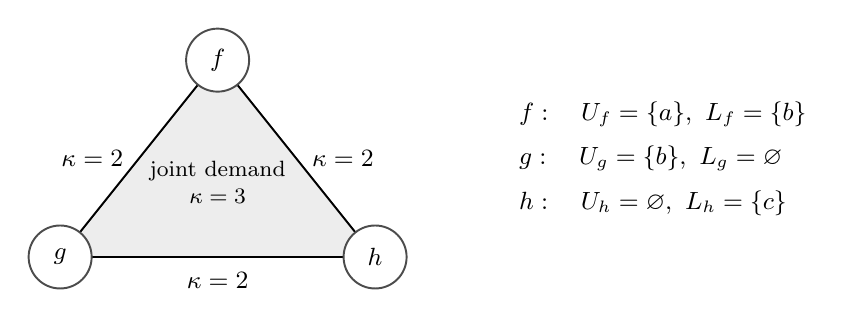
\begin{tikzpicture}[font=\small,every path/.style={line width=.7pt},
 world/.style={circle,draw=black!70,fill=white,minimum size=8mm,inner sep=1pt}]
\fill[black!7] (0,2.5) -- (-2,0) -- (2,0) -- cycle;
\draw (0,2.5) -- node[left,xshift=-2pt] {$\kappa=2$} (-2,0);
\draw (0,2.5) -- node[right,xshift=2pt] {$\kappa=2$} (2,0);
\draw (-2,0) -- node[below,yshift=-2pt] {$\kappa=2$} (2,0);
\node[world] at (0,2.5) {$f$};
\node[world] at (-2,0) {$g$};
\node[world] at (2,0) {$h$};
\node[align=center,font=\footnotesize] at (0,.95) {joint demand\\$\kappa=3$};
\node[anchor=west,align=left] at (3.7,1.25) {
  $f:\quad U_f=\{a\},\ L_f=\{b\}$\\[5pt]
  $g:\quad U_g=\{b\},\ L_g=\varnothing$\\[5pt]
  $h:\quad U_h=\varnothing,\ L_h=\{c\}$};
\end{tikzpicture}


\caption{A conflict involving three states at budget two. Each edge denotes
a feasible pair. The shaded triple is a minimal infeasible family. The late
quotas of $f$ and $h$ are one; the quota of $g$ is zero.}
\label{fig:conflict}
\end{figure}

\Needspace{11\baselineskip}
\begin{proposition}\label{prop:locality}
The threshold function need not be submodular and need not satisfy
LP-type locality.
\end{proposition}
\begin{proof}
Let $A=\{f\}$ and $B=\{f,g\}$ in~\eqref{eq:triple}. The marginal cost
of adding $h$ is zero on $A$ and one on $B$, violating the diminishing
returns inequality for submodularity.

LP-type locality requires that, whenever $A\subseteq B$ and
$\kappa(A)=\kappa(B)$, a state that strictly raises the value of $B$
also strictly raises the value of $A$~\cite{amenta,amentathesis}.
Here $\kappa(A)=\kappa(B)=2$, whereas adding $h$ raises only the value
of $B$.
\end{proof}

Short infeasibility certificates and locality are distinct properties
in the general theory~\cite{amentathesis}. The example identifies their
separation within the present resource objective: a continuation can
become costly through its interaction with another possible continuation.

\subsection{Resource budget and constraint-set cardinality}
For comparison, a family of sets, each of cardinality at most $k$, has
Helly number at most $k+1$~\cite[Theorem~7]{cardinal}. Our parameter
counts removal units. A state's feasible early plans can form a much
larger set: at budget two, a state with urgent set $\{a\}$ and no late
requests permits every plan $\{a,x\}$.

The distinction persists under alternative exact intersection
representations. Take four states with distinct urgent singletons,
no late requests, and budget two. Every pair is feasible and every
triple is infeasible. Suppose sets $S_1,\ldots,S_4$ represent this
feasibility pattern by nonempty intersections. Choose
$x_j\in S_1\cap S_j$ for $j=2,3,4$. These three points are distinct,
since an equality would give a point in three sets. Hence
$\card{S_1}\ge3$. Thus this budget-two example requires constraint
sets larger than two in any exact intersection representation.

\subsection{Actions that remove several targets}
\begin{proposition}\label{prop:area}
When one unit may remove several targets, minimal infeasible families
can have arbitrarily large cardinality at budget one.
\end{proposition}
\begin{proof}
Fix $n\ge2$ and take $n$ states, with urgent set $\{i\}$ in state $i$
and no late requests. For each $j$, provide an action $a_j$ that costs
one unit and removes all targets except $j$. Every proper subfamily
omits some state $j$ and is defended by $a_j$. No available action
defends the full family. Its cardinality is $n$, as required.
\end{proof}

The unit cost of an individual target is therefore the mechanism behind
Theorem~\ref{thm:helly}. It makes every additional indispensable urgent
requirement consume a separate part of the budget.

\section{Signals and minimal-obstruction hypergraphs}\label{sec:signals}

Fix a finite state space $\Omega\subseteq\Theta$ and budget $k$.
Define a hypergraph $\mathcal H_k$ on $\Omega$ whose edges are the
inclusion-minimal families $C$ with $\kappa(C)>k$. By
Theorem~\ref{thm:helly}, every edge has size at most $k+1$.
Under a uniform late reserve $d$ for $\Omega$, every edge has size at
most $1+\max\{k-d,0\}$.

Suppose an informed sender supplies a deterministic signal
$s:\Omega\to M$ with finite message alphabet $M$ before the early choice.
We count the messages in $s(\Omega)$; the empty state space uses zero
messages and has weak chromatic number zero. The defender then selects an
early set using the received message. The message class $s^{-1}(m)$
is exactly the set of states that this choice must jointly defend.

\begin{proposition}\label{prop:signal}
A signal permits guaranteed defense at budget $k$ if and only if no
edge of $\mathcal H_k$ is monochromatic. If every singleton is feasible,
the minimum number of messages equals the weak chromatic number of
$\mathcal H_k$.
\end{proposition}
\begin{proof}
A message class is feasible precisely when it contains no minimal
infeasible subfamily. Indeed, an infeasible finite class contains such
a subfamily, and any class containing one is infeasible by monotonicity.
Thus every message class is feasible exactly when no hyperedge lies
inside one class. This is the definition of a weak proper coloring.
If every singleton is feasible, assigning a separate message to each
state gives a proper coloring, so both minima exist and coincide.
\end{proof}

The use of common successful decisions to characterize information
classes is shared with hypergraph approaches to coding for function
computation~\cite{yuan}. Here the resource bounds control the sizes of
the minimal forbidden classes. In the example of~\eqref{eq:triple},
the sole minimal obstruction is the three-state set: any two states
may share a message, but all three may not. Pairwise conflict graphs
therefore omit an interaction that is decisive for successful signaling.

\section{Formalization and further questions}

The accompanying Lean sources formalize the exact threshold and its
minimum-budget interpretation (Theorem~\ref{thm:threshold}), monotonicity,
the witness-selection lemma, and both sharp obstruction bounds
(Theorems~\ref{thm:helly} and~\ref{thm:reserve}), including the singleton
case $d>k$. They also formalize the three-state values and the counterexamples
in Propositions~\ref{prop:locality} and~\ref{prop:area}. Safety universally
quantifies over admissible late target sets. The proofs derive maximum
late demand, establish the optimality of the urgent union, and select
target witnesses. The sequential interpretation, private-target argument,
intersection representation, and signal-coloring correspondence have the
direct proofs given above.

One direction is to characterize the minimal-obstruction hypergraphs of
removal models. Such a characterization
would describe the information partitions compatible with a given resource
budget. A second direction allows heterogeneous costs or multiple urgent
deadlines; the monotonicity identity~\eqref{eq:cost} identifies an exchange
property to examine in those settings. Card effects that alter target
accessibility or remove several targets also provide concrete settings for
studying how interruption granularity changes the order of hidden-state conflicts.

\subsection*{Declaration of AI assistance}
GPT-6 Astra assisted with the mathematical derivations in this paper.

\Needspace{26\baselineskip}
\begin{thebibliography}{10}
\raggedright

\bibitem{amenta}
Nina Amenta, \emph{Helly-type theorems and generalized linear programming},
Discrete \& Computational Geometry \textbf{12} (1994), 241--261.
\url{https://www.cs.ucdavis.edu/~amenta/pubs/helly.pdf}.

\bibitem{amentathesis}
Annamaria Beatrice Amenta, \emph{Helly Theorems and Generalized Linear Programming},
Ph.D. thesis, University of California, Berkeley, 1993.
\url{https://www.cs.ucdavis.edu/~amenta/pubs/ninathesis.pdf}.

\bibitem{cardinal}
Jean Cardinal, Hiro Ito, Matias Korman, and Stefan Langerman,
\emph{Helly numbers of polyominoes}, Proceedings of the 23rd Canadian
Conference on Computational Geometry, 2011.
\url{https://cccg.ca/proceedings/2011/papers/paper104.pdf}.

\bibitem{goerigk}
Marc Goerigk, Stefan Lendl, and Lasse Wulf,
\emph{Two-stage robust optimization problems with two-stage uncertainty},
arXiv:2104.03043, 2021. \url{https://arxiv.org/abs/2104.03043}.

\bibitem{kasperski}
Adam Kasperski and Pawe{\l} Zieli{\'n}ski,
\emph{Robust recoverable and two-stage selection problems},
arXiv:1505.06893, 2015. \url{https://arxiv.org/abs/1505.06893}.

\bibitem{konami}
Konami Digital Entertainment, \emph{Yu-Gi-Oh! card database},
English and Japanese card entries.
\url{https://www.db.yugioh-card.com/yugiohdb/}.

\bibitem{timing}
Konami Digital Entertainment, \emph{Fast effect timing}.
\url{https://www.yugioh-card.com/en/play/fast-effect-timing/}.

\bibitem{yuan}
Deheng Yuan, Tao Guo, Bo Bai, and Wei Han,
\emph{Lossy computing with side information via multi-hypergraphs},
arXiv:2205.08262, 2022. \url{https://arxiv.org/abs/2205.08262}.

\end{thebibliography}
\end{document}
